\paragraph{Conditional initialization checks.}
With data and shuffle order fixed and parent-selected learning rates frozen, Cora / GCN gives mean validation-selected test loss 0.8807 for QuotientOpt and 1.1376 for AdamW, a 22.6\% reduction over three model initializations; QuotientOpt has lower test loss in 3/3 paired initializations.
With data and shuffle order fixed and parent-selected learning rates frozen, SDF / SIREN gives mean validation-selected test loss $1.10\!\times\!10^{-5}$ for QuotientOpt and $6.21\!\times\!10^{-5}$ for AdamW, a 82.2\% reduction over three model initializations; QuotientOpt has lower test loss in 3/3 paired initializations.
All four methods, individual outcomes, and initialization SDs are reported in Appendix~\ref{app:initialization-confirmation}. These checks quantify conditional variability across the stated initializations on a fixed split and do not create independent data-set replications.
\begin{figure}[t]
\centering
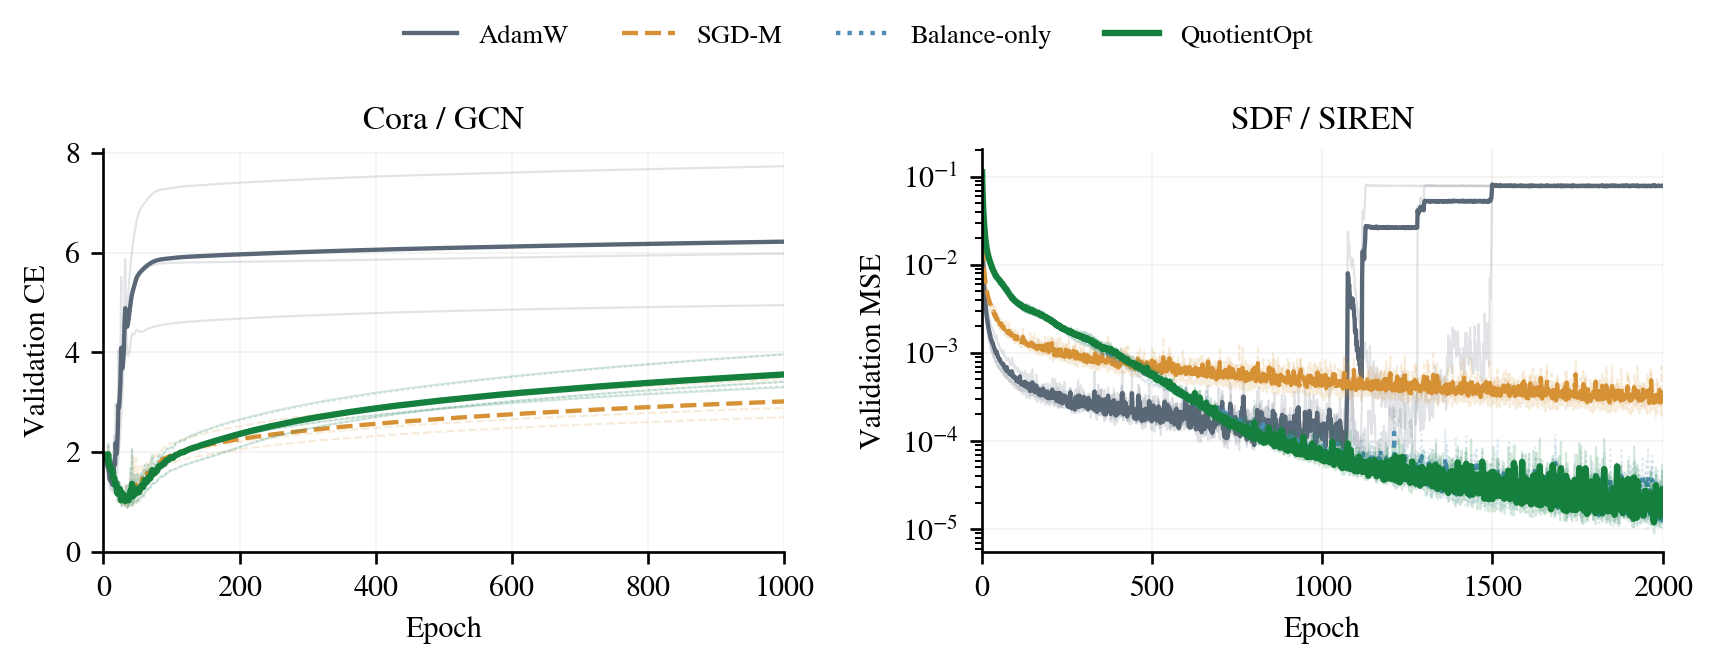
\includegraphics[width=.99\linewidth]{figures/initialization_confirmation_curves.png}
\caption{\textbf{Conditional initialization loss checks.} Data and shuffle seed 42 are fixed, with model initializations 42, 43, and 44. Parent-selected learning rates are frozen per method, with no per-initialization retuning. Thin lines show every initialization; thick lines show their arithmetic mean validation loss at each epoch. All raw epochs are retained without smoothing. The mean curves are descriptive summaries, not confidence bands. Test outcomes and all four controls are retained in Table~\ref{tab:initialization-confirmation}.}
\label{fig:initialization-loss}
\end{figure}
